\documentclass{article}
\usepackage[utf8]{inputenc}
\usepackage[T1]{fontenc}
\usepackage{lmodern}


\usepackage{csquotes}
\usepackage[brazilian]{babel}

\usepackage{graphicx}
\usepackage{indentfirst}
\usepackage[inline]{enumitem}
\usepackage{outlines}
%\setlist{nolistsep}
\setlist{nosep}
\renewcommand{\labelitemi}{$\bullet$}
\renewcommand{\labelitemii}{$\circ$}
\renewcommand{\labelitemiii}{$\diamond$}
\renewcommand{\labelitemiv}{$\circ$}
% Bibliografia deve ser construida com um arquivo 
% no formato BibLaTeX (levemente diferente do BibTeX)
\usepackage[citestyle=numeric,
%articlein=false,style=ext-authoryear-comp,
natbib=true]{biblatex}
% pode simplesmente trocar o nome do seu arquivo aqui
\addbibresource{ementabiblio.bib}

\usepackage{coisas}

\usepackage{hyperref}
\hypersetup{hidelinks,colorlinks = false}
\PassOptionsToPackage{hyphens}{url}




\title{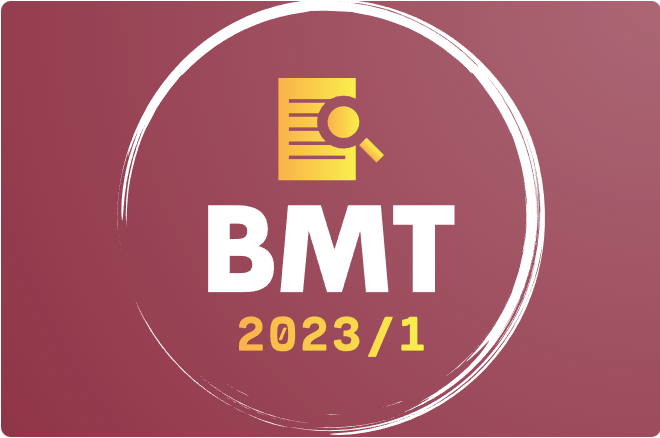
\includegraphics[width=0.3\textwidth]{images/logobmt.png}~ 
\\[1cm]
CPS738 - Busca e Mineração de Texto}
\author{Geraldo Xexéo}
\date{Período: 2023/01}


\begin{document}

\maketitle

\section{Apresentação do Curso}

O curso de Busca e Mineração de Texto tem como objetivo introduzir os alunos às práticas de processamento de texto e linguagem natural, com base nas soluções para o  problema da Busca e Recuperação da Informação (BRI), e mostrando como as mesmas técnicas são a base para a área de Mineração de Texto (MT).

A cadeira busca dar um entendimento de:
\begin{outline}
\1 O que é um texto, um documento e como são suas representações digitais.
\1 Como são as técnicas de pré-processamento de texto e documentos para a indexação, busca e mineração de texto.
\1 Como funciona um mecanismo tradicional de BRI.
\1 Como funcionam as técnicas tradicionais de MT.
\1 Como funcionam as técnicas de Redes Neurais Profundas (DNN), incluindo os conceitos de Seq2Seq, Aprendizado por Transferência, Transformadores e Atenção, para MT.
\end{outline}

Boa parte do curso será guiada pelo livro em construção ``Tópicos em Busca da Informação e Mineração de Texto''. 

\section{Informações Gerais}
\begin{itemize}
    \item Nome do Curso: Busca e Mineração de Texto
    \item Código COPPE: COS738 (3 créditos)
    \item Outros Códigos: Alunos de graduação da ECI podem usar uma cadeira de Tópicos Especiais ou tentar Bancos de Dados Avançados
    \item Professor: Geraldo Xexéo
    \item Horário: A determinar
    \item Local: A Determinar
    \item WhatsApp de participação obrigatória: \url{https://chat.whatsapp.com/GCtUBmL0YaoKte9w6UktI2}
\end{itemize}

Esse curso aceitará matrícula de alunos de graduação da ECI, ECA e DCC.

\section{Objetivo}

Após o curso o aluno deverá ser capaz de participar da construção de ferramentas que realizam o fluxo de trabalho completo de BRI e MT, a partir de ferramentas de software disponíveis no mercado, compreender os algoritmos utilizados, seus impactos e como implementar seus próprios algoritmos, juntando o conhecimento do curso aos conhecimentos anteriores de programação.

\section{Pré-Requisitos}

Os alunos devem programar com desenvoltura. 

O curso é baseado em Python, onde é recomendado conhecimento prévio, e KNIME, onde não é necessário conhecimento prévio. Alguns exemplos podem usar a linguagem Java. 

Alunos com algum conhecimento de Aprendizado de Máquina e Redes Neurais terão mais facilidade no curso, porém os tópicos introdutórios necessários para esses assuntos serão cobertos. 

\section{Competências Esperadas ao Final do Curso}



\begin{outline}
    \1 Compreender como um texto é representado de forma digital, incluindo os conceitos de conjunto de caracteres e formato de arquivos.
    \1 Implementar a leitura de arquivos em vários formatos por meio de ferramentas disponíveis,
    \1 Compreender a forma geral de funcionamento de um mecanismo de BRI.
    \1 Compreender o conceito de relevância.
    \2 Compreender o funcionamento dos modelos traducionais de BRI> booleano, vetorial e probabilístico.
    \1 Aplicar diferentes modelos de BRI, incluindo o  booleano, vetorial, o modelo LSI e o modelo de linguagem.
    \1 Compreender o funcionamento do \textit{feedback} de relevância.
    \1 Aplicar as formas de avaliação de mecanismos de BRI.
    \1 Compreender como avaliar um experimento de Aprendizado de Máquina.
    \1 Compreender as limitações de BRI, incluindo questões de escala e relevância.
    \1 Aplicar ferramentas de software existentes para o processamento de texto.
    \1 Compreender o conceito de Classificação e Agrupamento por Aprendizado de Máquina 
    \1 Planejar experimentos de Mineração de Texto.
    \1 Implementar sistemas simplificados de BRI.
    \1 Explicar o funcionamento dos principais modelos de MT. 
    \1 Elaborar experimentos de Mineração de Texto.
    
\end{outline}


\section{Metodologia}

A principal metodologia utilizada será a de aulas expositivas e presenciais, seguidas de propostas de trabalhos práticos.

Além disso, os alunos se dividirão em grupos que realização um trabalho de cadeira, cujo tema e escopo será acordado com o professor.

Ao longo do curso poderão ser usadas aulas remotas ou aulas gravadas para o estudo de material complementar.

\section{Política de Avaliação}

A avaliação será baseada em:
\begin{outline}
    \1 Trabalhos práticos, de programação, individuais (50\% da nota). Esses trabalhos são entregues por meio do Moodle. Os trabalhos previstos (pode haver modificação) são:
    \2 Processar um documento XML (prática de auto-aprendizado)
    \2 Detecção da codificação de arquivo
    \2 Implementação de um sistema de recuperação em memória segundo o modelo vetorial
    \2 Avaliação do mecanismo de busca implementado
    \2 Classificação de documentos por aprendizado supervisionado 
    \1 Trabalho em grupo, constando de um artigo, com implementação. Exemplos dos artigos esperados podem ser vistos em \citep{xexeo2022} (50\% da nota). Esse trabalho deve ser entregue uma semana após a última aula, por meio do Moodle.
\end{outline}

\section{Política de Presença}

A presença é obrigatória, sendo a reprovação automática em função da quantidade de faltas segundo as normas da UFRJ.

\section{Ementa}

\begin{outline}
\1 Parte Introdutória~\citep{xexeo2023}
\2 Textos e Documentos. Codificação de Caracteres. Processamento de Arquivos Textuais~\citep{xexeo2023}. 
\1 Pré-Processamento e Algoritmos Básicos~\citep{xexeo2023,jurafsky2022}.
\2 Morfologia. Tokenização. \textit{Case Folding}. Stemming. \textit{Stop-words}. Normalização. Estruturas Chave-Valor. Lista Invertida. Caches. Tabela de Espalhamento. 
\1 Busca e Recuperação da Informação.
\2 Medidas de Avaliação. Relevância. \textit{Aboutness}, Recuperação. Softwares de Full-Text Search. Modelo Booleano. Modelo Vetorial. Modelo Probabilístico. BM25. Indexação por Semântica Latente. Modelos de Linguagem. Arquitetura de Mecanismos de Busca~\citep{Baeza2011}.
\1 Mineração de Texto~\citep{jurafsky2022}
\2 Aprendizado de Máquina.
  Algoritmos de
Classificação. Algoritmos de Agrupamento. Redes Neurais. Redes Neurais Profundas. Transformadores. Atenção. Embeddings. BERT.  
\1 Aplicações
\2 Tag Clouds~\citep{Morgado2010,xexeo2022,xexeo2023}. Análise de Sentimentos. Crawlers. Recursos Lexicais. Detecção de Plágio~\citep{Abreu2011,Duarte2017}. 
\end{outline}
\section{Recursos Disponíveis}

    Entre os recursos disponíveis estão:
    \begin{outline}
        
    
        \1 Slides de todas as aulas
        \1 Coleções de dados para os exercícios individuais
        \1 Material de auto-aprendizado para assuntos que são pré-requisitos para o curso
        \1 Bibliografia de referência, com artigos e etc.
        \1 Um livro em construção pelo professor, que é referência do curso
    \end{outline}

 Todo material do curso estará disponível em \url{http://moodle.cos.ufrj.br}
 
 Além disso, há um grupo de WhatsApp de participação obrigatória \url{https://chat.whatsapp.com/GCtUBmL0YaoKte9w6UktI2}


\section{Contato com o professor}

O meio de contato prioritário com o professor é o grupo de WhatsApp. Todo o contato relacionado a assuntos da matéria e prazos deve ser feito no grupo e de forma pública.

Outros contatos podem ser feitos pelo e-mail (\url{mailto:xexeo@cos.ufrj.br}) ou diretamente pelo WhatsApp do professor, principalmente em casos mais pessoais.

Não há horário de atendimento previsto fora da sala de aula, porém eles podem ser marcados pelo grupo de WhatsApp e pelo e-mail do professor.

\section{Alunos com Necessidades Especiais}

Alunos com necessidades especiais devem entrar em contato com o professor para as providências necessárias, incluindo PcD ou outras necessicidades. 

\section{Plano de Aulas}

O plano de aulas atualizado pode ser encontrado no Moodle. Os assuntos previstos são:

\begin{outline}
    \1 Introdução
    \2 Introdução ao Curso
    \2 O que é Texto
    \2 Codificação de Caracteres
    \2 Aprendizado de Máquina
    \2 Lei de Zipf
    \2 Formatos de Documetnos
    \2 Modelos Conceituais para Documentos
    \1 Pré-Processamento
    \2 Introdução ao Pré-Processamento
    \2 Stop Words
    \2 Stemming
    \1 XML (auto-aprendizado)
    \1 Relevância
    \1 Tarefas e Modelos de IR
    \1 Modelo Booleano
    \1 Modelo Vetorial
    \2 Introdução ao Modelo Vetorial
    \2 TF-IDF
    \2 Modelo Vetorial para Documentos Longos
    \2 Relevance Feedback
    \1 Modelo Probabilístico
    \1 Avaliação de um Mecanismo de Busca
    \1 Modelos Avançados de IR
    \2 Modelo de Semântica Latente
    \2 Language Models
    \1 Hits, Pagerank e BrowseRank
    \1 Expressões Regulares (auto-aprendizado)
    \1 POS-Tagging
    \2 Etiquetadores
    \2 HMM e MEMM    
    \1 Spell-Checking
    \1 Plágio
    \1 Fingerprints e LSH
    \1 Arquitetura de um Mecanismo de Busca
    \1 Semântica de Vetores e Embeddings
    \1 Introdução a Linguística Computacional
    \1 KNIME
    \1 Tranformadores e Atenção
    \1 BERT e \textit{Transfer Learning}
    \1 Pytorch
    \1 RNN e LSTM
    \1 Extração da Informação
    \1 Reconhecimento de Entidades Nomeadas
    \1 Sumarização
\end{outline}


\nocite{*}
\printbibliography
\end{document}
